Training the model with different sizes of latent dimensions yielded some different results, in different aspects of the task the model had. Below can we see how the loss differ from each other: \\

\begin{figure}[!ht]
  \centering
  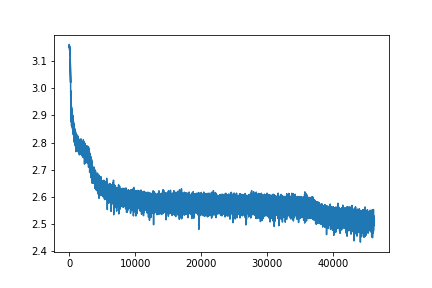
\includegraphics[width=0.4\linewidth]{latex/imgs/CNN_loss_latent_dimension_100.png}
  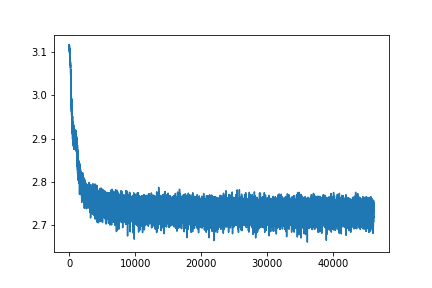
\includegraphics[width=0.4\linewidth]{latex/imgs/loss_latent_dimension_50.png}
  \caption{losses of the of cnn trained with latent dimension $4$x$100$(left) and $2$x$50$(right)}
  \label{fig:cnn_loss}
\end{figure}

\noindent
As can be seen on the graph (figure ~\ref{fig:cnn_loss}), the one with a high latent dimension had a noticeably better loss, than the one with a lower latent dimension. Which makes good sense, since the model with a greater latent dimension has more data to use in the reconstruction. Since the loss was based on the model's ability to reconstruct the image; it is no surprise that the one with higher dimensionality reduction, had better reconstruction accuracy.

\begin{table}[!ht]
\centering
\begin{tabular}{|l|l|l|}
\hline
 latent\_dimension: & $4$x$100$  &  $2$x$50$ \\ \hline
min\_loss model     & 0.2039 & 0.1473 \\ \hline
fully trained model & 0.2058 & 0.1469 \\ \hline
\end{tabular}
\caption{reconstruction accuracy}
\end{table}

\noindent
It's important to note, that the reconstruction accuracy is not defining how well the model is performing on the separation task or the spearmen correlation.\\

\noindent
The following figures (figure ~\ref{fig:plot_50} and ~\ref{fig:plot_100}) show the structural plotting of the model's latent representation run through a t-sne. As can be seen, on the figures. The model seems to find some separation between the different structural classes. As can be seen, both models find some separation between classes (C, B, G) with some overlapping. The rest of the classes is mostly spread out between the groups. Indicating that this model is not very good at finding much structural separation. \\

\begin{figure}[!ht]
  \centering
  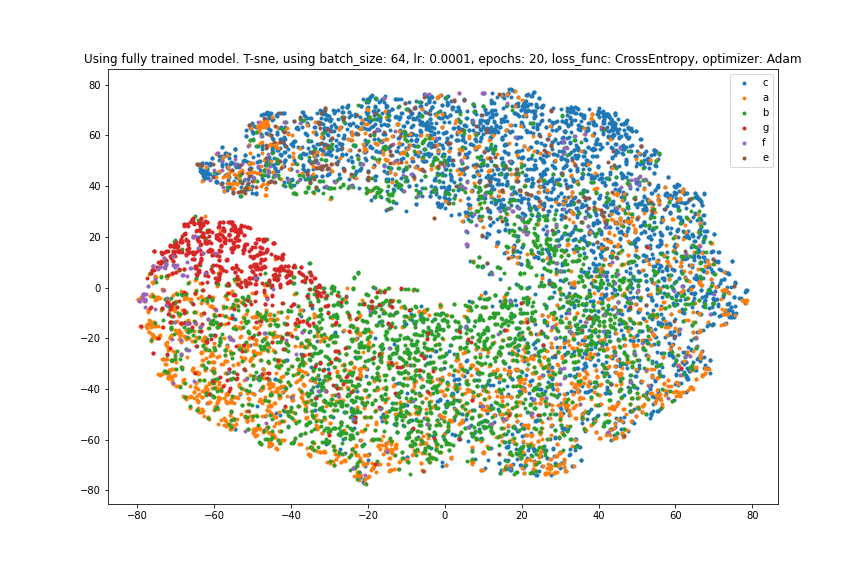
\includegraphics[width=0.4\linewidth]{latex/imgs/last_50.png}
  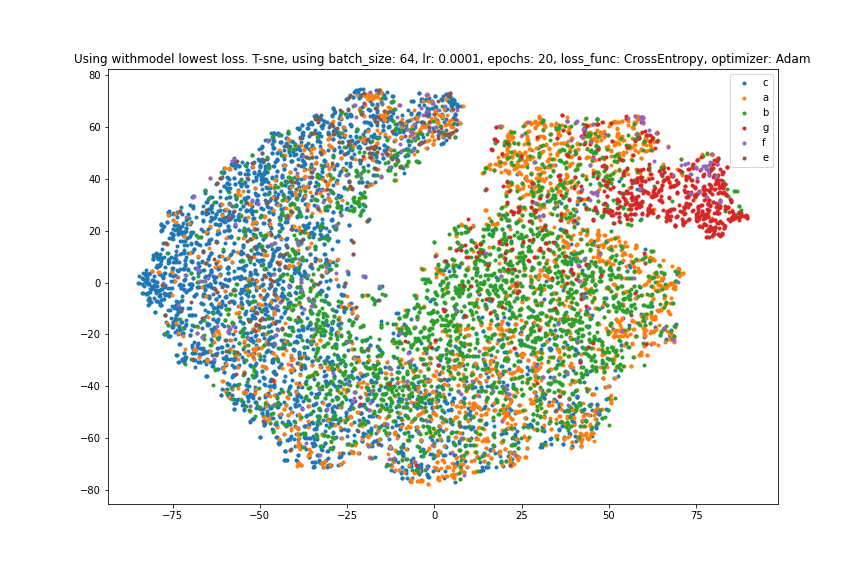
\includegraphics[width=0.4\linewidth]{latex/imgs/best_50.png}
  \caption{plot showing secondary structure seperation with latent dimension $2$x$50$. Fully trained model(left), min loss model (left)}
  \label{fig:plot_50}
\end{figure}

\begin{figure}[!ht]
  \centering
  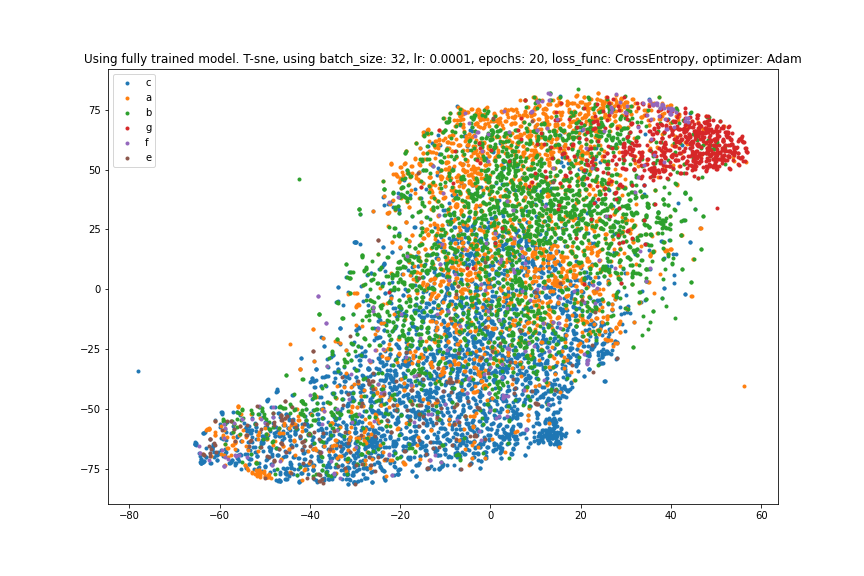
\includegraphics[width=0.4\linewidth]{latex/imgs/last_100.png}
  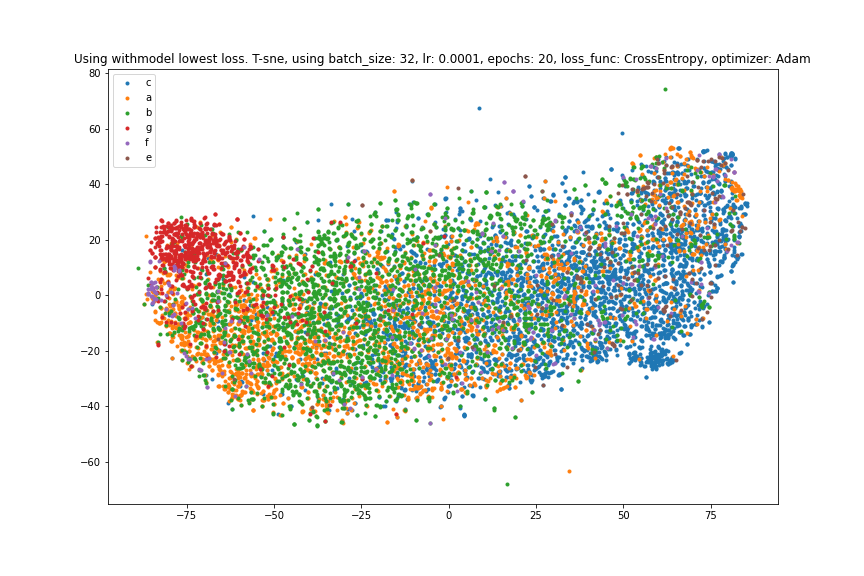
\includegraphics[width=0.4\linewidth]{latex/imgs/best_100.png}
  \caption{plot showing secondary structure seperation with latent dimension $4$x$100$. Fully trained model(left), min loss model (left)}
  \label{fig:plot_100}
\end{figure}

\noindent
The two figures (figure ~\ref{fig:stab_100} and ~\ref{fig:stab_50}) yielded the following results on the stability dataset calculating spearment correlation.


\begin{figure}[!ht]
  \centering
  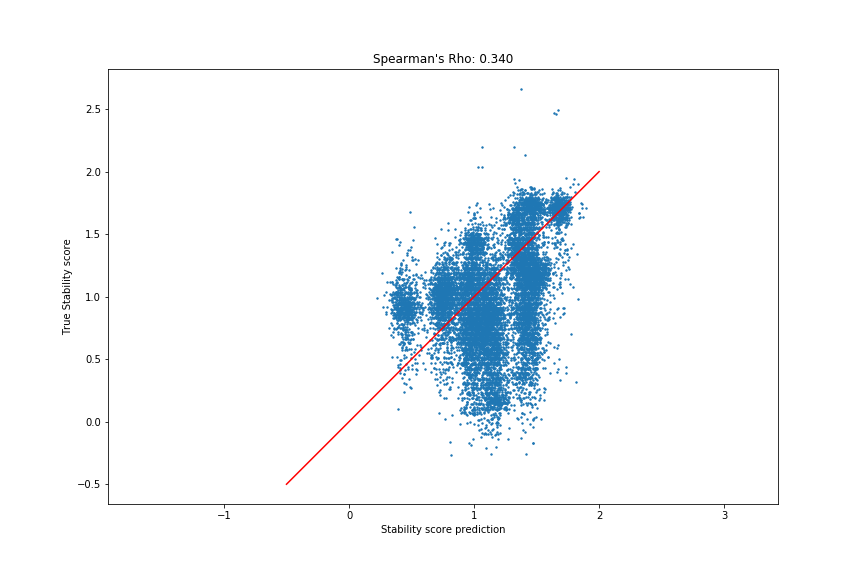
\includegraphics[width=0.4\linewidth]{latex/imgs/CNN_spearman_correlation_100_fully.png}
  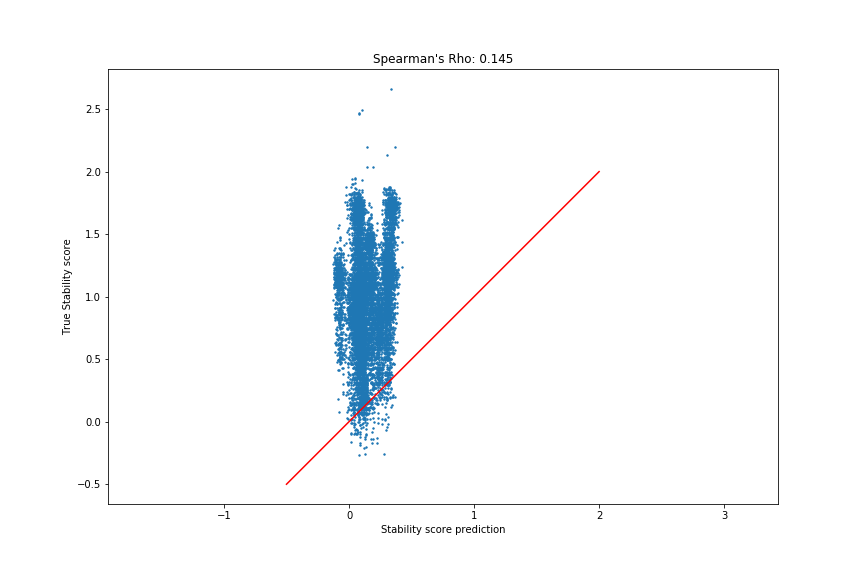
\includegraphics[width=0.4\linewidth]{latex/imgs/CNN_spearman_correlation_100_best.png}
  \caption{Graph showing the spearman correlation from model with latent dimension $4$x$100$. Fully trained model(left), min loss model (left)}
  \label{fig:stab_100}
\end{figure}

\begin{figure}[!ht]
  \centering
  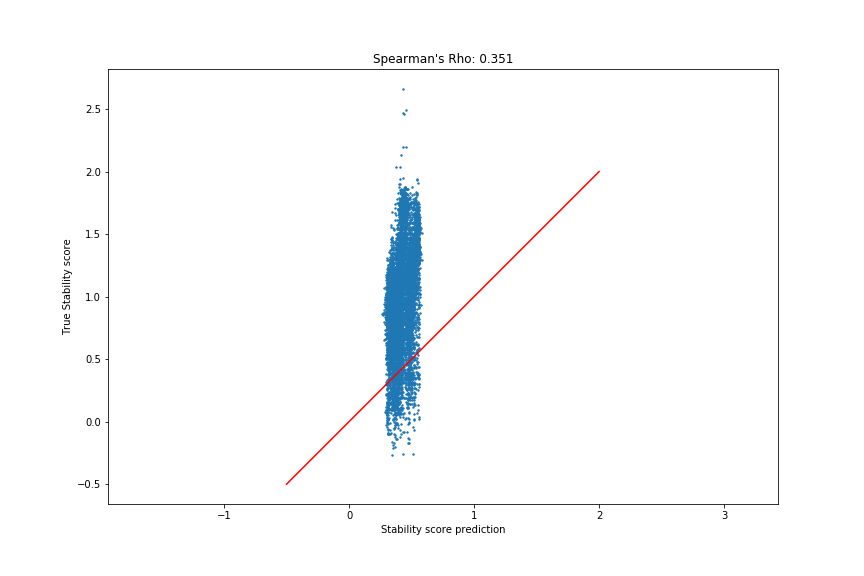
\includegraphics[width=0.4\linewidth]{latex/imgs/CNN_spearman_correlation_50_fully.png}
  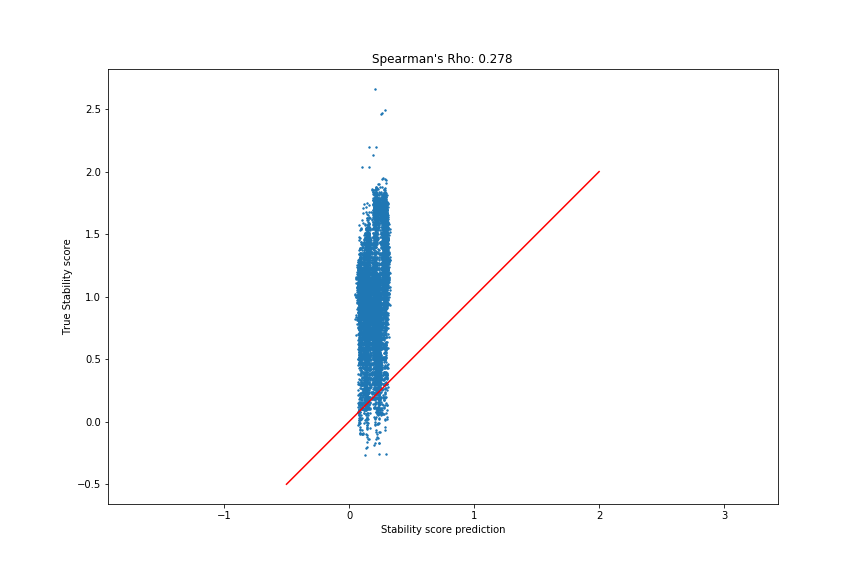
\includegraphics[width=0.4\linewidth]{latex/imgs/CNN_spearman_correlation_50_best.png}
  \caption{Graph showing the spearman correlation from model with latent dimension $2$x$50$. Fully trained model(left), min loss model (left)}
  \label{fig:stab_50}
\end{figure}

\noindent
It would seem that the model converges at about 0.3, which not especially great results since they are pretty far from the optimal results 1. Yet, it means that the model has learned some representation of the structure. \\

\noindent
In general in these experiments, the results from the minimum loss model, doesn't perform that different compared to the fully trained model.